%LTeX: language=pt-br
% !TeX root = Apostila_IM381.tex

\cleardoublepage
\section{Considerações e propriedades}

    Nesta seção, serão discutidas algumas fontes de erros no Método de Elementos Finitos, assim como algumas considerações adicionais que devem ser levadas em conta ao realizar a análise numérica.

    Conforme apresentado nas seções anteriores, o MEF é um método numérico no qual obtemos uma solução aproximada do problema analisado. Desta forma, erros aparecem na solução. Há várias fontes de erro que podem poluir o resultado, e conhecê-las nos auxilia na interpretação dos valores obtidos. Conhecê-las também nos permite ter uma confiabilidade maior no método, assim como diagnosticar as causas de erros nos resultados.

    Em problemas complexos, sem solução analítica bem definida, não há nenhuma garantia de solução exata. Na verdade, nestes casos, espera-se que nunca cheguemos precisamente na solução exata, erros sempre estarão inclusos no nosso resultado. Estes podem ser dividos nas seguintes categorias:

    \subsubsection*{Erros de modelagem}

        Antes de aplicar o MEF, precisamos de um modelo matemático representativo do sistema. Estes erros provêm da diferença entre o comportamento real e o modelo matemático adotado.

        Por exemplo, um modelo de material linear elástico isotrópico e homogêneo será representativo para um aço. Entretanto, a depender do tratamento térmico, pode ser que este material perca sua isotropia, e o modelo deixe de representar adequadamente o sistema real. Um polímero também terá erros consideráveis se utilizarmos este modelo, exigindo a aplicação de modelos constitutivos de materiais hiperelásticos.

        

        Outros exemplos de erros de modelagem que se inserem aqui são: aplicação indevida de modelos de pequenas deformações ou pequenos deslocamentos, imprecisões nas aproximações das condições de contorno do sistema. Representação aproximada das cargas impostas no sistema.

        Para corrigir estes erros, é necessário que o engenheiro tenha a capacidade de discernimento sobre o quão adequado é cada modelo para aquela aplicação específica, visto que modelos mais complexos exigem um maior custo computacional.

    \subsubsection*{Erros de discretização}

        Conforme estudado nas seções anteriores, o MEF é um método numérico no qual obtemos uma solução aproximada para a função incógnita. Esta pode ser um campo de temperatura, campo de potencial elétrico, campo de deslocamentos, entre outros.

        Esta função incógnita pertence a um espaço $V$ de dimensão infinita. A priori, deconhecemos quem deve ser esta função solução, inclusive, está pode nem ser análitica, basta que ela pertença a $V$. O MEF aproxima a solução para um espaço de dimensão finita $V^h$, obtendo a função deste espaço que melhor se aproxima da exata.

        Os erros de discretização provêm da diferença entre a solução exata e a solução aproximada obtida. Em casos particulares, como barras, eixos, vigas e placas, é possível que esta diferença seja zero. Entretanto, de forma geral, sempre haverá um erro, não importa o quanto aumentemos a dimensão de $V^h$, isto é, não importa o quanto aumentemos o número de funções de forma, refinando a malha em mais elementos finitos. A Figura \ref{fig:discretizacao_erro} ilustra este erro, mostrando a diferença entre as deformações e deslocamentos de um problema de barra.

        \begin{figure}[h!]
            \begin{subfigure}{0.9\textwidth}
                \centering
                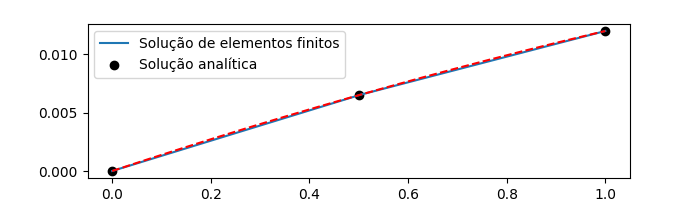
\includegraphics[scale=0.9]{Figures/4-Elemento_barra/Deslocamento_exemplo_4-1.png}
                \caption{}
            \end{subfigure}\\
            \begin{subfigure}{0.9\textwidth}
                \centering
                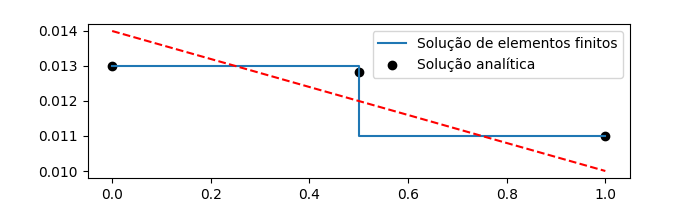
\includegraphics[scale=0.9]{Figures/4-Elemento_barra/Deformacao_exemplo_4-1.png}
                \caption{}
            \end{subfigure}
            \caption{Erros de discretização em barra. (a) Deslocamento, (b) deformação}
            \label{fig:discretizacao_erro}
        \end{figure}

        Este erro também inclui imprecisões sobre a geometria do domínio, como mostrado na Figura \ref{fig:modelo_erro}. Muitas vezes, os elementos adotados não se encaixam perfeitamente na geometria, e a superfície do modelo passa a ser uma aproximação da geometria real.

        \begin{figure}[h!]
            \centering
            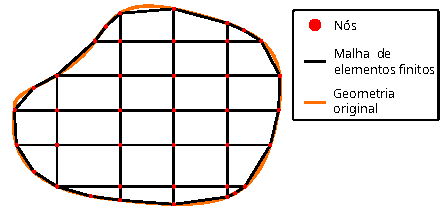
\includegraphics[scale=1]{Figures/4-Elemento_barra/Malha.pdf}
            \caption{Discretização de uma geometria em elementos finitos}
            \label{fig:modelo_erro}
        \end{figure}

    \subsubsection*{Erros de truncamento}

    Um computador salva os números como variáveis que ocupam certas estruturas específicas. Por exemplo, um valor pode ser salvo como uma variável inteira \textit{int} ou \textit{long}. Ambos salvam variáveis inteiras, porém, a diferença entre elas é a sua precisão, isto é, o tamanho dos números que estas são capazes de armazenar. Para armazenar variáveis com uma precisão superior, é necessário utilizar um espaço maior da memória.

    Para variáveis reais, de forma geral, utiliza-se o tipo \textit{float} ou \textit{double}. Nas linguagens C/C++, a primeira utiliza 4 bytes de memória para armazenar por volta de 7 algarismos significativos, a segunda ocupa 8 bytes e armazena por volta de 15 algarismos. No Python, o tipo chamado \textit{float} na verdade corresponde ao \textit{double} da linguagem C.

    As variáveis \textit{float} e \textit{double} aloca números sempre em notação científica em base binária. Nesta notação, qualquer número será da seguinte forma:

    \begin{equation}
        \textit{num. binário em notação científica} = 1, \square \times 10^\square
    \end{equation}

    Por exemplo:

    \begin{equation*}
        65.25 = 1000001.01 = 1.00000101 \times 10^6
    \end{equation*}

    \begin{equation*}
        -0.171875 = -0.001011 = -1.011 \times 10^{-3}
    \end{equation*}

    Portanto, devem ser salvas três informações: o sinal, o expoente e a mantissa (dígitos que aparecem após a vírgula).

    Um \textit{double} possui 8 bytes, isto é, 64 bits (lembrando que 1 byte possui 8 bits). Um bit é a unidade de armazenamento em um computador, e armazena um dado de forma binária, isto é, pode estar ativado (1) ou desativado (0). O sinal é armazenado em 1 bit, representando positivo ou negativo. O expoente é representado em 11 bits, e a mantissa nos últimos 52 bits. Caso o número seja irracional ou uma dízima periódica (na base binária!), então este será truncado e representado de forma aproximada na memória.

     \begin{lstlisting}[language=C++]
        /**
            Exemplo de erros devido a precisao numerica
            em codigo em C
        **/

        // Pi salvo em float
        float pi_float = 3.1415927;

        // Pi salvo em double
        double pi_double = 3.141592653589793;

    \end{lstlisting}

    \subsubsection*{Erros de manipulação numérica}

    Ainda no contexto do erro de truncamento, como as variáveis são truncadas, podem aparecer erros em determinadas operações devido a este truncamento:

    \begin{lstlisting}[language=Python]
        # Exemplo de erros em Python

        print(2.1 * 7)
        # >> 14.700000000000001
        # 2.1 em binario: 10.0001100110011001101
        # Dizima periodica em binario!

        print(1.000000000000001 - 1)
        # >> 1.1102230246251565e-15
        
        print(1 + 1e-16 - 1)
        # >> 0.0

    \end{lstlisting}

    Principalmente em operações que devem ser muito próximas de zero, pode aparecer um erro significativo na resposta. Se, por sua vez, este valor estiver, por exemplo, no denominador de uma divisão, isso pode levar a uma explosão no erro numérico associado a essa operação. Por esta causa, normalmente os métodos numéricos evitam operar com divisões de números pequenos. Um exemplo disso é na solução de sistemas lineares, no qual é feita uma permutação na etapa de pivotamento, para reduzir este tipo de erro.

    Além disso, podemos perder informação significativa para o resultado se somarmos ou subtrairmos dois números com ordens de grandeza muito distintas:

    \begin{lstlisting}[language=Python]
        # Exemplo de erros em Python

        print(1 + 1e-16 - 1)
        # >> 0.0

        print(1 -1 + 1e-16)
        # >> 1e-16

        print(1.000000000000001 -1 + 1e-16)
        # >> 1.2102230246251566e-15

    \end{lstlisting}

    Portanto, também evita-se operar números com esta característica. Se possível, podemos alterar a ordem das operações para reduzir erros, entretanto, esta troca ainda pode trazer os erros citados acima.



    \subsection{Condicionamento de uma matriz}

        No MEF, obtemos uma matriz, chamada matriz de rigidez. Esta matriz, junto com o vetor de forças, resulta no campo de deslocamentos nodais. Desta forma, a matriz de rigidez carrega toda a informação do problema analisado. Portanto, é essencial garantir que esta matriz carregue adequadamente estas informações. Para isso, usaremos algumas propriedades da Álgebra Linear.

        Uma matriz, no contexto do espaço vetorial dos vetores euclidianos, é um tensor. Isto é, ela representa uma transformação linear aplicada a um vetor. A Figura \ref{fig:transformacao_linear} ilustra essa operação. O vetor $\bm{u}$ sofre uma transformação linear pela aplicação do tensor $\bm{T}$, resultando no vetor $\bm{v}$. Matematicamente:

        \begin{equation}
            \bm{v} = \bm{T} \bm{u}
        \end{equation}

        \begin{figure}[h!]
            \centering
            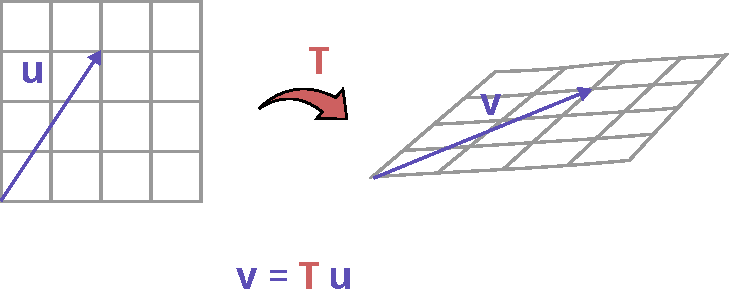
\includegraphics[scale=1]{Figures/10-Consideracoes/Matriz.pdf}
            \caption{Aplicação de uma transformação linear. O espaço se distorce após está, e o vetor muda de direção e módulo.}
            \label{fig:transformacao_linear}
        \end{figure}

        O condicionamento de uma matriz mede o quão sensível o vetor resultante $\bm{v}$ é à uma perturbação no vetor inicial $\bm{u}$. Uma matriz é dita bem condicionada se ele é pouco sensível. Em uma matriz mal condicionada, a solução é bastante sensível a pequenas perturbações. A Figura \ref{fig:mal_condicionado} ilustra uma transformação descrita por uma matriz mal condicionada.

        \begin{figure}[h!]
            \centering
            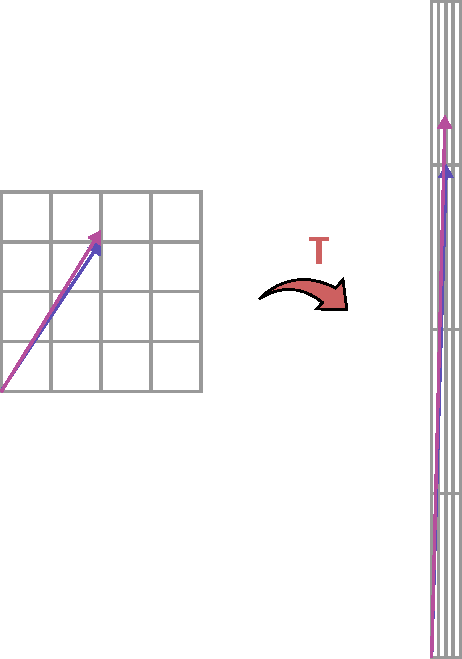
\includegraphics[scale=1]{Figures/10-Consideracoes/Matriz_condicionamento.pdf}
            \caption{Aplicação de uma transformação linear mal condicionada.}
            \label{fig:mal_condicionado}
        \end{figure}

        Um sistema linear representado por uma matriz mal condicionada apresenta uma sensibilidade maior a perturbações nos valores da matriz.

        Vamos verificar essa sensibilidade com um exemplo, abaixo:

        \begin{equation}
            \begin{bmatrix}
                1 & -1\\
                -1 & 1+a
            \end{bmatrix}
            \begin{Bmatrix}
                x_1\\
                x_2
            \end{Bmatrix}
            =
            \begin{Bmatrix}
                4\\
                -2
            \end{Bmatrix}
        \end{equation}

        Se resolvermos este sistema, chegamos a seguinte solução:

        \begin{equation}
            \begin{Bmatrix}
                x_1\\
                x_2
            \end{Bmatrix}
            =
            \begin{Bmatrix}
                4+\frac{2}{a}\\
                \frac{2}{a}
            \end{Bmatrix}
        \end{equation}

        Vamos agora adotar valores para $a$ para observar 

        \begin{equation}
            a =0,01
            \rightarrow
            \begin{Bmatrix}
                x_1\\
                x_2
            \end{Bmatrix}
            =
            \begin{Bmatrix}
                204\\
                200
            \end{Bmatrix}
        \end{equation}

        \begin{equation}
            a =0,009
            \rightarrow
            \begin{Bmatrix}
                x_1\\
                x_2
            \end{Bmatrix}
            =
            \begin{Bmatrix}
                226,2\\
                222,2
            \end{Bmatrix}
        \end{equation}

        Uma pequena variação no valor de $a$ resultou em uma diferença expressiva na resposta. Perceba que esta diferença representa uma mudança de $1,01$ para $1,009$ no termo da matriz, uma variação de menos de 1\% no valor.

        Na prática, em problemas computacionais, conforme mostrado anteriormente, teremos erros de truncamento associados às operações de máquina. Visto a inevitabilidade desses erros, desejamos matrizes bem condicionadas, para evitar que estes sejam amplificados demasiadamente.

        \subsubsection*{Exemplo: molas em série}

            Para ilustrar o efeito do mau condicionamento de uma matriz, considere o sistema da Figura \ref{fig:molas}, composto por duas molas em série, com rigidezes $k_1$ e $k_2$. A mola de rigidez $k_2$ está presa em uma parede fixa, a outra está sujeita a uma força $F$. A equação de equilíbrio deste sistema é dado por:

            \begin{equation}
                \begin{bmatrix}
                    k_1 & -k_1\\
                    -k_1 & k_1 + k_2
                \end{bmatrix}
                \begin{Bmatrix}
                    u_1\\
                    u_2
                \end{Bmatrix}
                =
                \begin{Bmatrix}
                    F\\
                    0
                \end{Bmatrix}
            \end{equation}

            \begin{figure}[h!]
                \centering
                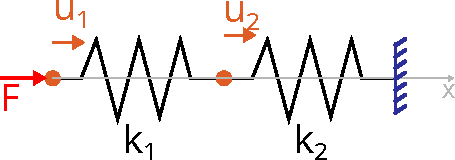
\includegraphics[scale=1]{Figures/10-Consideracoes/Molas.pdf}
                \caption{Molas em série}
                \label{fig:molas}
            \end{figure}

            Resolvendo este sistema, chegamos nos deslocamentos:

            \begin{equation}
                u_1 = \frac{F}{k_1} + \frac{F}{k_2} \quad , \quad  u_2 = \frac{F}{k_2}
            \end{equation}

            Suponha agora, que $k_2 \gg k_1$. Quando realizamos a operação $k_1 + k_2$, se o segundo for muito maior que o primeiro, devido à precisão de máquina, teremos apenas $k_1 + k_2 \approx k_2$:

            \begin{equation}
                \begin{bmatrix}
                    k_1 & -k_1\\
                    -k_1 & k_2
                \end{bmatrix}
                \begin{Bmatrix}
                    u_1\\
                    u_2
                \end{Bmatrix}
                =
                \begin{Bmatrix}
                    F\\
                    0
                \end{Bmatrix}
            \end{equation}

            Este sistema será resolvido normalmente, resultando em:

            \begin{equation}
                u_1 \approx \frac{F}{k_1} + \frac{F}{k_2} \quad , \quad  
                u_2 = \frac{F}{k_2-k_1} \approx \frac{F}{k_2}
            \end{equation}

            Desta forma, o resultado permanece satisfatório, dentro de uma precisão aceitável.

            Agora, suponha que $k_1 \gg k_2$. Pelo mesmo motivo que anteriormente, o valor de $k_1$ significativamente superior a $k_2$ o ofuscará, resultando em:

            \begin{equation}
                \begin{bmatrix}
                    k_1 & -k_1\\
                    -k_1 & k_1
                \end{bmatrix}
                \begin{Bmatrix}
                    u_1\\
                    u_2
                \end{Bmatrix}
                =
                \begin{Bmatrix}
                    F\\
                    0
                \end{Bmatrix}
            \end{equation}

            Este sistema possui infinitas soluções, pois a matriz é singular. Portanto, no caso extremo no qual $k_2$ não aparece de forma alguma na matriz, o computador será inclusive incapaz de resolver o sistema!

            Este caso nos ilustra que devemos nos atentar a variações muito grandes de propriedades de material dentro do sistema, especialmente se isso inclui partes muito flexíveis nas regiões de condições de contorno.

        \subsubsection*{Análise de autovalores}

            Uma matriz quadrada pode ser descrita também pelos seus autovalores e autovetores. Os autovalores $\lambda$ e autovetores $\bm{v}$ de uma matriz $\bm{K}$, são pares escalar-vetor que satisfazem:

            \begin{equation}
                \bm{K}\bm{v} = \lambda \bm{v}
            \end{equation}

            Matrizes hermitianas (que é o caso em MEF) possuem $n$ pares de autovalores e autovetores, no qual $n$ é o tamanho da matriz.

            Graficamente, os autovetores de uma matriz representam as direções que não se alteram após a transformação linear. Isto é, qualquer vetor na direção de um autovetor $\bm{v}_i$ continua na mesma direção após a transformação (Figura \ref{fig:autovalor}). Os autovalores representam o fator de escala aplicado a vetores nestas direções.

            \begin{figure}[h!]
                \centering
                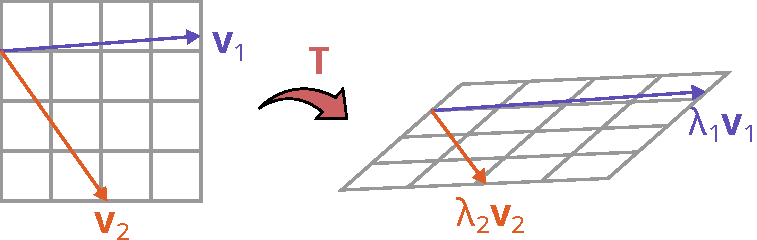
\includegraphics[scale=1]{Figures/10-Consideracoes/Autovalor.pdf}
                \caption{Autovalores e autovetores de uma transformação linear}
                \label{fig:autovalor}
            \end{figure}

            Matrizes de rigidez em elementos finitos (após aplicação das condições de contorno) são positivo definidas, isto é:

            \begin{equation}
                \lambda_i > 0
            \end{equation}

            Um vetor qualquer no espaço $n$ dimensional pode ser escrito como uma combinação linear dos autovetores. Por exemplo, para $n = 2$:

            \begin{equation}
                \bm{u} = a_1 \bm{v}_1 + a_2 \bm{v}_2
            \end{equation}

            \begin{equation}
                \bm{K}\bm{u} 
                = a_1 \lambda_1 \bm{v}_1 + a_2 \lambda_2 \bm{v}_2 
                = \lambda_1 \left( a_1 \bm{v}_1 + a_2 \frac{\lambda_2}{\lambda_1} \bm{v}_2\right)
            \end{equation}

            Entretanto, se $\lambda_1 \gg \lambda_2$, assim como no exemplo da mola, podemos perder informações na resposta, visto que $\frac{\lambda_2}{\lambda_1} \approx 0$:

            \begin{equation}
                \bm{K}\bm{u} 
                \approx a_1 \lambda_1 \bm{v}_1
            \end{equation}

            Portanto, se o autovetor associados aos autovalores pequenos tiverem uma contribuição significativa na composição de $\bm{u}$, podemos perder informações significativas sobre este. Importante salientar que isso indica apenas uma \textbf{possível} perda de precisão na resposta, isso não significa que efetivamente \textbf{teremos} a precisão afetada.

            Para medir a possível perda de precisão na resposta, define-se o número de condicionamento:

            \begin{equation}
                C(\bm{K}) = \frac{\lambda_\text{max}}{\lambda_\text{min}}
            \end{equation}

            \noindent no qual $\lambda_\text{max}$ e $\lambda_\text{min}$ são, respectivamente, o maior e o menor autovalor da matriz $\bm{K}$.

            Um número de condicionamento elevado está, usualmente associado a perda de informação no autovetor associado ao menor autovalor. Na prática, pode-se utilizar a seguinte expressão:

            \begin{equation}
                \text{perda de precisão} \approx \text{log}_{10} C(\bm{K}) = \text{log}_{10} \frac{\lambda_\text{max}}{\lambda_\text{min}}
            \end{equation}

            \noindent no qual a perda de precisão é o número de casas decimais (a partir da menor) nos quais há erros numéricos.

    \subsection{Refino p e h}

    \subsection{Singularidades}
